\documentclass[fleqn,10pt]{wlscirep}
\usepackage[utf8]{inputenc}
\usepackage[T1]{fontenc}
\usepackage{listings}
\title{Odysseia: Genetic Regulatory Feature Analysis with Interpretable Classification Machine Learning Models}

\author[1,*1]{Jack Yu}
% \author[1,2,*1]{Jack Yu}
\author[1,]{Jiawang Tao}
% \author[1,*2]{Jie Wang}

% \author[2,+]{Derek Author}
\affil[1]{Affiliation, department, city, postcode, country}
% \affil[2]{Affiliation, department, city, postcode, country}
\affil[*1]{Correspondence: gyu17@alumni.jh.edu}
% \affil[*2]{Correspondence: wang_jie01@gibh.ac.cn}
% \affil[+]{these authors contributed equally to this work}
\keywords{Cell Reprogramming, Machine Learning, Gene Regulatory Network}

\begin{abstract}
With rapid progress of robust single-cell transcriptome sequencing since last decade, numerous complex mechanisms underlying cell development has been revealed.
Single-cell RNA sequencing (scRNA-seq) analysis is widely accepted as the main approach to define cell stages and phenotypes.
As conversion of somatic cells into induced pluripotency cells succeeded, identification key genetic factors(GFs) with scRNA-seq for cell reprogramming in biological research and regenerative medicine fields gained increasing attention.
Herein, we describe \emph{Odysseia}, an interpretable machine learning classifier based single-cell gene expression profile(scGEP) analysis system, that assesses importances of genetic regulatory features in differentiating cell state(CS).
Furthermore, extracted factors, when combining with regulatory network analysis, can help to find key GFs in classifying CSs and possibly implementing CS conversions.
\emph{Odysseia} correctly extracted GFs acclaimed to be capable of inducing CS conversion in three published cell reprogramming related studies on different cell types, including [embryonic stem cells(ESC), myogenic progenitor cell(MPC), and neurons]!!!please double check this part. 
Overall, \emph{Odysseia} provides an automated alternative to obtain guidance information while elucidating mechanism to engineer cellular phenotypes.
\end{abstract}

\begin{document}
\flushbottom
\maketitle
% * <john.hammersley@gmail.com> 2015-02-09T12:07:31.197Z:
%
%  Click the title above to edit the author information and abstract
%
\thispagestyle{empty}
% \noindent Please note: Abbreviations should be introduced at the first mention in the main text – no abbreviations lists. Suggested structure of main text (not enforced) is provided below.
\section*{Introduction}
Since cell reprogramming of mouse embryonic fibroblasts(MEF) to induced pluripotent stem cell(iPSC) succeed in 2006\cite{yamanaka_2006}, several more CS transition methods have been established both \emph{in vivo} and \emph{in vitro}\cite{fibroblast_sertoli_2012,fibro_cardio_2012,mef_hept_2011}, spurring prospective development in biomedical area.
However, reprogrammed cells may fail to match precisely in vivo counterparts' identities\cite{ASCL1_dopaminergic_neuron_2021}, and precise reprogramming toward cell subtypes remains impossible\cite{cell_repro_review}.
As gene expression profiles for each individual cell in query population became accessible with scRNA-seq, substantial progress in accurately defining cell subtypes with marker gene expression has been made\cite{pancreas_subtypes_2016,lung_subtypes_2014}.
Even though multiple computational methods, like \emph{CellNet}\cite{cellnet_2014}, method of \emph{D’Alessio et al}\cite{dalessio_2015}, and \emph{Mogrify}\cite{mogrify_2016}, are informative of determining key transcription factors(TFs) for CS conversion via carrying out novel human cell conversion experiments, limited generalized method could achieve similar goal while utilizing scRNA-seq based expression profiles instead of microarray based or Cap analysis gene expression (CAGE) based databases.
Indeed, constructing scRNA-seq based gene expression database is possible to expand existing methods' applicability in predicting key TFs for cell subtype conversions and elucidating detailed mechanism behind cell reprogramming.
Maintaining complicated database covering majority discovered cell subtypes require massive work; hence, developing generalized scRNA-seq based predictive computational method for determining key GFs in CS conversion with existing methods remain challenging.
In 2019, \emph{SingleCellNet}\cite{scn_2019} was published as successor of \emph{CellNet} in classifying cellular samples with scRNA-seq data but not guiding CS conversion.

Here we present \emph{Odysseia}, a set of scRNA-seq based expression profile analysis system utilizing interpretable machine learning classifiers, for  guiding CS conversion method design and elucidating mechanisms behind CS conversions.
Unlike previous described methods, \emph{Odysseia} does not require any background expression database but searching for potential key GFs by inverting one CS to another with only expression profiles labeled with binary CS categories as input.
Genetic regulatory pathways(GRPs) contributing to classifying CS category classification will be addressed through assessing and interpreting trained classifiers.
Then, key genes that induces CS conversion will be addressed through analyzing regulons constructed with GRPs described above.
This design is based on the knowledge that the key genes and GRPs may not have converged profiles in either expression or regulatory aspects.
Classification model designed to directly find CS deterministic genes or GRPs may fail to converge on a stable solution.
One of the intuitive approach to solve the non-convergence issue is transforming classification question into higher dimension.
Therefore, instead of asking which factors are CS deterministic, we determined CS category, a converged and labeled profile among input data, with given GEP.
Then, we analyzed the well-performing classifiers and found features, equivalent to GRPs, essential for the classifiers to make correct decisions.

However, if features associated with similar functions are sufficiently informative, CS classifiers could reach remarkably high accuracy with a small number of heavily-weighted features.
As a result, potential key features will presumably be lost even classifiers demonstrated high accuracy over testing data, and output informativity will be impaired.

For example, cell differentiation or cell type transformation is accompanied by a series of GEP and epigenetic changes, processes usually occur during the cell cycle.\cite{dalton_2015, engstrom_2021}
As a result, GFs related to cell cycle or proliferation can be used as differential characteristics to classify CSs but are not key regulators of the differentiation process.
If only these GFs are found after classifier analysis, system output's capability in guiding CS conversion may not be sufficient.
Therefore, a particular classification model designed solving transformed question can still encounter feature lost issue.

In order to overcome feature lost issue, \emph{Odysseia} applies multiple classification models with distinct architecture settings in each training iteration then selects well-performing classifiers for further assessment and interpretation.
Through interpreting top-performing classifiers trained with different batches of input data, \emph{Odysseia} enhances the feature extraction capability.

The {\hyperref[method]{\textbf{Method}}} section explains the overall system design. The {\hyperref[res]{\textbf{Result}}} section shows package performance on three existing datasets with high fidelity. At last, further experiments and potential improvements is discussed in the {\hyperref[disc]{\textbf{Discussion}}} section. 


\section*{Methods}
\label{method}
Briefly, \emph{Odysseia} consists of 4 main steps as shown in Figure \ref{odysseia}:
\begin{itemize}
  \item \hyperref[step1]{\textbf{\emph{Step 1}}}: Generate pseudo-celluar gene expression profiles(pseudo-cGEPs) and corresponding pseudo-cellular genetic regulatory network(pseudo-cGRN) with genetic regulatory network(GRN) reconstruction guidance.
  \item \hyperref[step2]{\textbf{\emph{Step 2}}}: Train classification models with GRNs reconstructed with pseudo-cGEPs then select out well-performing models via accuracy evaluation.
  \item \hyperref[step3]{\textbf{\emph{Step 3}}}: Interpret selected classifiers' correct predictions on all generated GRNs.
  \item \hyperref[step4]{\textbf{\emph{Step 4}}}: Perform regulon based analysis on important GRPs found from classifer interpretation in step 3 and extract key genes indicated by the GRPs.
\end{itemize}


\begin{figure}[ht]
\centering
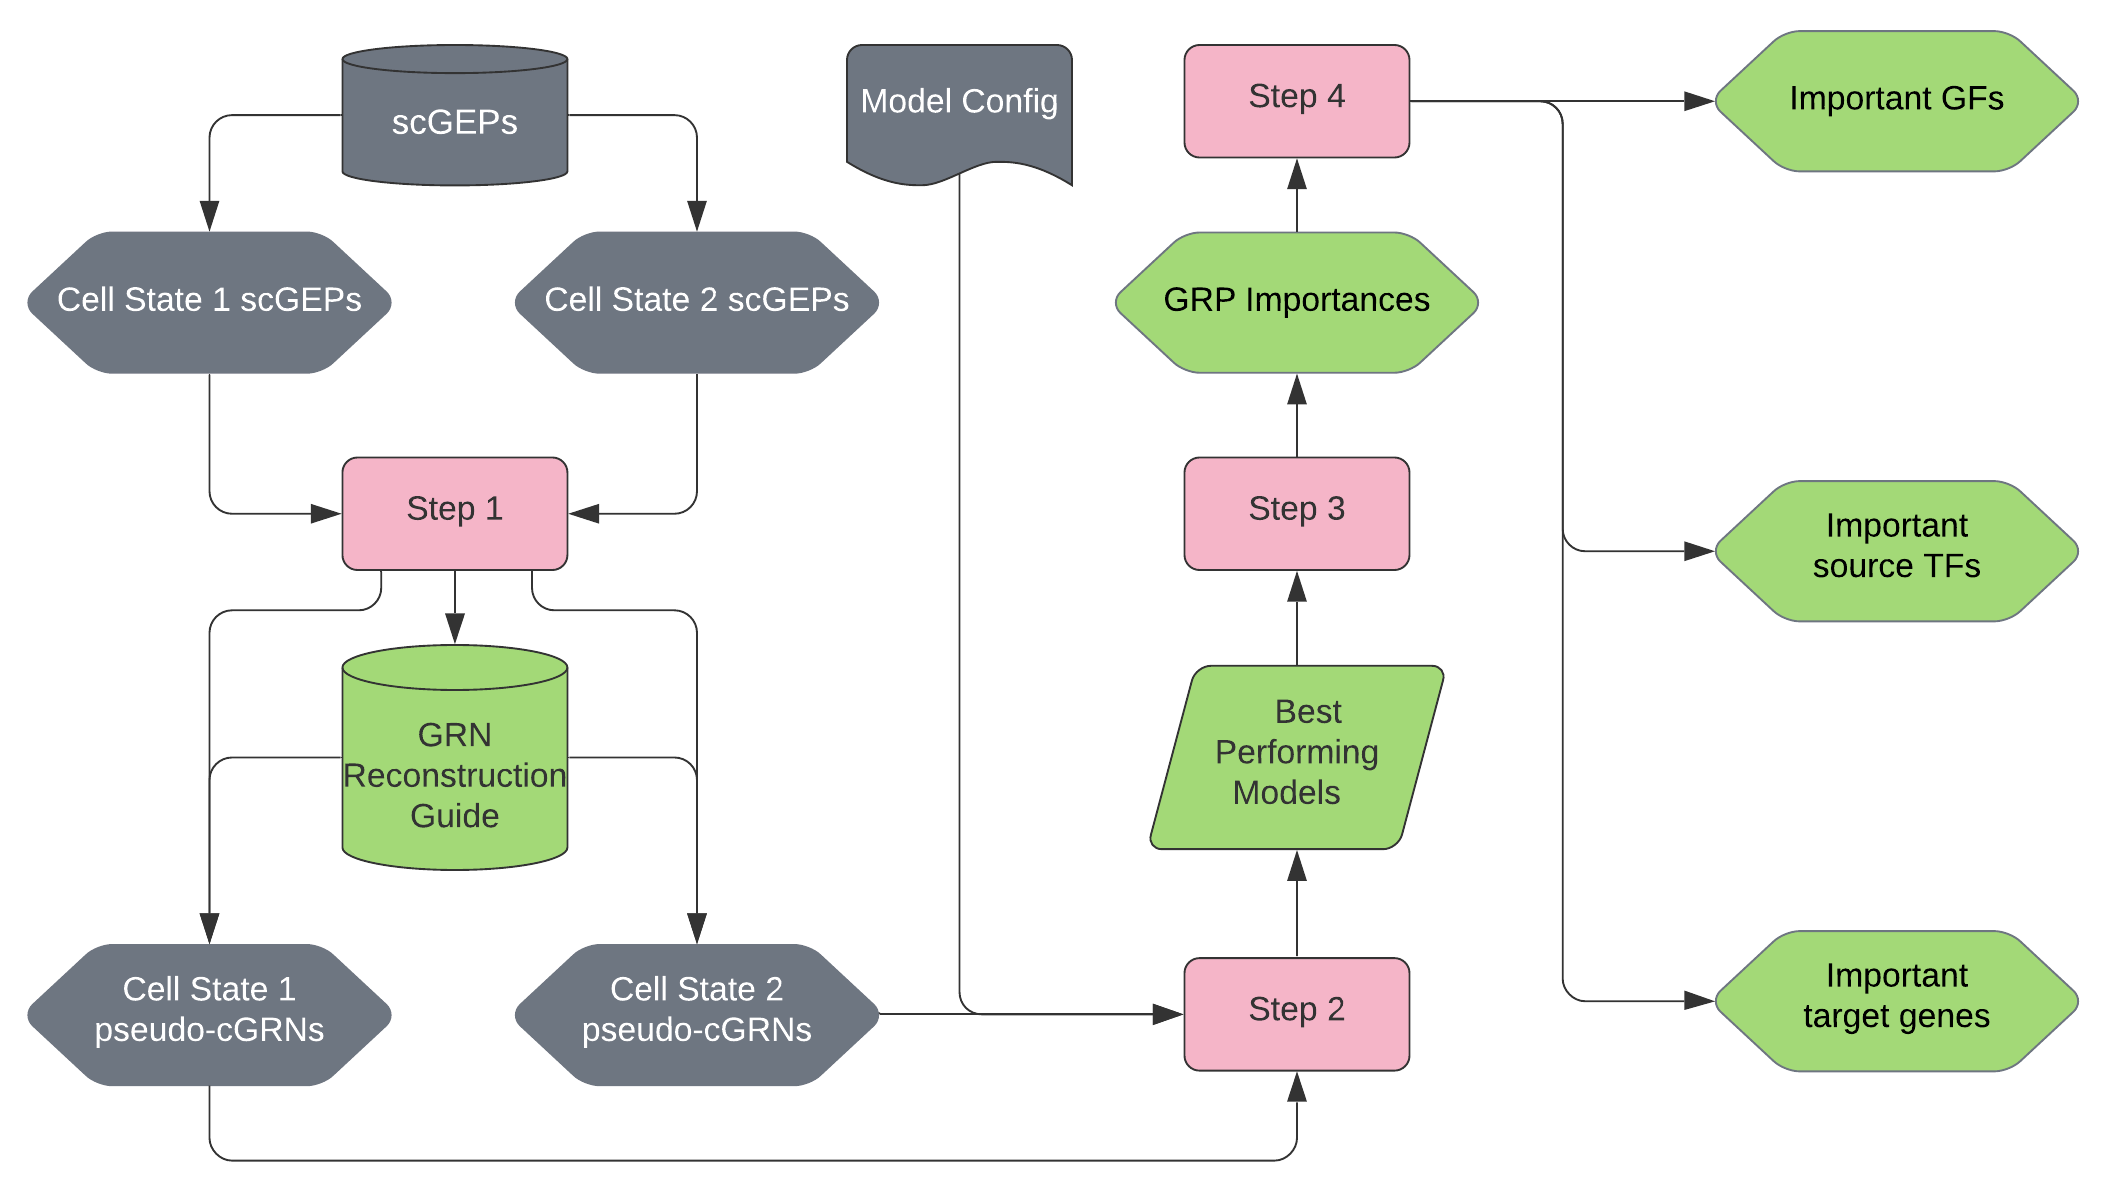
\includegraphics[width=0.8\linewidth]{image/Odysseia.png}
\caption{The overall workflow of \emph{Odysseia}}
\label{odysseia}
\end{figure}


\subsection*{Step 1: Data pre-processing}
\label{step1}
A computational method measuring iteration strength among gene pairs is used to reconstruct GRNs based on scGEPs.
One of the widely adopted methods is Pearson's Correlation coefficient(PCC)\cite{cid_2019, pcc_2012}.
Sequence of expression levels(ELs) for each gene among iteration is calculated.
Hence, in order to reconstruct cell-level GRNs, \emph{Odysseia} segments scGEPs under same CS category into subsets with constant size to form pseudo CEPs, having gene ELs gained from different cells abstracted as sequence of altering ELs among single pseudo cell???.

With scarce scGEPs, sliding window algorithm(SWA) with customized window size and padding stride can be applied to ensure sufficient pseudo-cGEP for later classifier training and assessment processes. With SWA, \emph{i-th} pseudo-cGEP can be obtained through:

\centerline{$SWA(i) = \left\{{x_j}_{j = i * s}^{j + l}\right\}, j + l < N$}
$N$ denotes total length of scGEPs gained from scRNA-seq, and scRNA-seq can be expressed as $\left\{{x_j}_{j = 0}^{N}\right\}$; $l$ denotes window size; $s$ denotes padding stride.

A meta-level process on determining gene pairs that form regulatory relationships in each pseudo-cGRN dramatically reduces computational resource requirement than repeatedly testifying all possible gene pairs in every pseudo-cGEP.
Assuming that pseudo-cGEPs have similar expression pattern with comprehensive GEP containing all scGEPs, the GRN reconstruction guidance can be created through analyzing all gene pairs in comprehensive GEP.
The overall workflow to create GRN reconsturction guidance is summarized in Figure \ref{kirke}.
In total, two sets of filters are used for validating a GRP:
\begin{enumerate}
\setlength\itemsep{0em}
\item {\textbf{Gene level}}:

The filter set below determines binary CS category differentiability of single gene expression pattern. 
\begin{itemize}
\setlength\itemsep{0em}
\item \textbf{Std Filter}: 
The Std of gene’s EL must be significant. Query gene reaches relatively high EL and its expression pattern can interact with other GFs. Std threshold is set to 1 by default, implying that only genes with expression status changing in different circumstances can be considered. In reality, Std threshold is adjusted in response to expression change weight and computational resource capacity. 

\item \textbf{MWU Filter}: The expression distribution of selected gene across samples labeled with different CSs must be dissimilar.
This filter aims to confirm that query gene's GEP is likely distinguishable across sample sets under binary CS categories.
The Mann-Whitney U rank test(MWU) implemented by \emph{SciPy}\cite{2020SciPy-NMeth} will be performed on GEPs of selected gene in binary CS categories.
The p-value for rejecting null hypothesis, that expression pattern underlying CS1 is the same as the expression pattern underlying CS2, is set to 0.05 by default.
\end{itemize}

\item {\textbf{Pathway level}}:

The filter set below determines the biological interpretability and significance of GRP. 
\begin{itemize}
\setlength\itemsep{0em}
\item \textbf{TF Filter}: The source input of a GRP must be a recorded TF.
If not further specified, TF list will be retrieved from integrated \emph{TRANSFAC}\cite{transfac} datasets according to the species information in query.
\item \textbf{GRP Filter}: Regulatory target must have binding ability with source TF. If not further specified, regulatory gene list of given TF will be retrieved from integrated \emph{GTRD}\cite{gkaa1057} datasets according to the species information in query.
\item \textbf{PCC Filter}: Expression correlation between source TF and target gene must be significant. The absolute value threshold  of Pearson correlation coefficient is 0.2 by default, as calculated with \emph{SciPy}\cite{2020SciPy-NMeth}.
\end{itemize}
\end{enumerate}
% In the case of not knowing source $TF's$ correlated binding site information, $GRNBoost2$\cite{grnboost2}-like algorithm will be initiated to predict potential regulatory target.
% The prediction process can either take manually set significant threshold or automatically set threshold based on validated GRPs.
% The process of automated prediction threshold setting can be expressed as:

% \centerline{$Threshold = min(G(E_1, t)\, \uplus \, G(E_2, t))$}

% \noindent Here $G()$ is GRNBoost2\cite{grnboost2}-like algorithm; $E_1$ is subtracted $CL1\;EM$ for GFs passed Gene level filters; $E_2$ is subtracted $CL2\;EM$ for GFs passed Gene level filters; $t$ is the regulatory source $TF$ in most amount of validated GRPs.
\begin{figure}[ht]
\centering
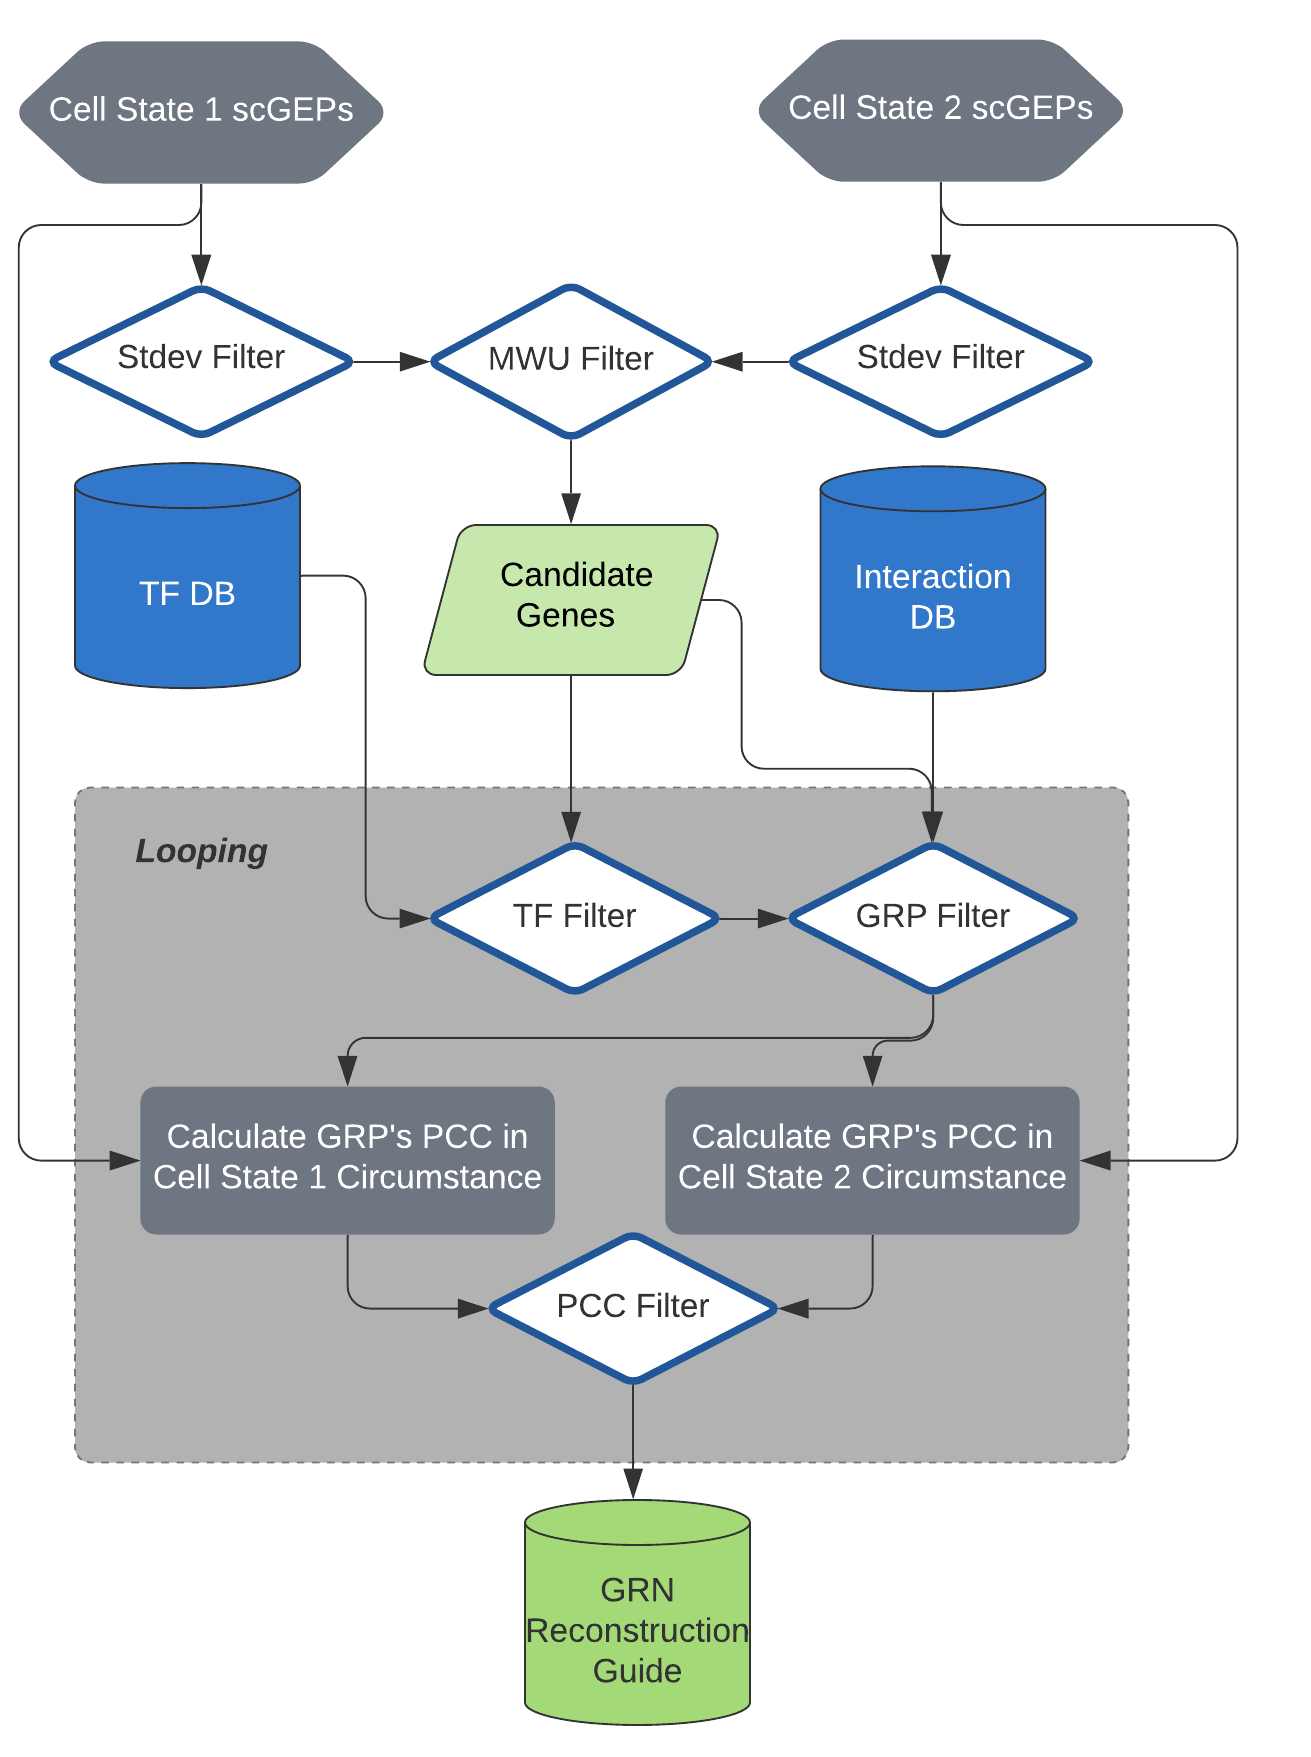
\includegraphics[width=0.8\linewidth, height=12cm, keepaspectratio,]{image/Kirke.png}
\caption{
Workflow to create GRN reconstruction guidance from comprehensive GEPs.
\textbf{\emph{(1)}} Each gene in scGEP set either for CS1 or CS2 need to pass Std filter to confirm its expression pattern reacts with inconstant gene expression circumstances.
\textbf{\emph{(2)}} GEPs of genes passed Std filter will be inputted to MWU filter to confirm that its gene expression pattern is differentiable among binary CS categories.
\textbf{\emph{(3)}} All TFs in genes passed MWU filter will be selected out as potential regulatory source TF utilizing given TF database.
\textbf{\emph{(4)}} Using GF or protein-protein interaction databae, all genes passed MWU filter will be testified as target genes with potential TF found at previous step to form potential interacting gene pairs.
\textbf{\emph{(5)}}, PCCs of potential interacting gene pairs found previously will be calculated under each CS category. A gene pair must have corresponding PCC under at least one CS category greater than the threshold to be considered as potential GRP.
}
\label{kirke}
\end{figure}

Utilizing GRN reconstruction guidance, pseudo-cGRN will be reconstructed for each pseudo-cGEP.
Each gene in the guidance, if also presents in pseudo-cGEP, need to pass the Std filter in pseudo-cGEP circumstance before validating correspond GRPs in the guidance.
The pre-validated GRPs that also passes PCC filter will take part in eventual pseudo-cGRN.

\subsection*{Step 2: Classifier selection}
\label{step2}
According to given model config file, vanilla models will be initialized with specified model type and architecture parameters.
\emph{Odysseia} will perform accuracy tests systematically aiming to select out potentially well-performing models for further analysis, while iterativly training classifiers with split pseudo-cGRN sets.
The overall workflow is summarized in Figure \ref{odysseus}.
Currently, \emph{Odysseia} supports three types of classification models:
\begin{itemize}
\setlength\itemsep{0em}
\item \textbf{SVC}: Support Vector Classifer implemented with \emph{scikit-learn}.\cite{scikit-learn}
All parameters adjustable with \emph{scikit-learn}\cite{scikit-learn} are supported.
\item \textbf{GBTree}: Gradient Boosting Trees implemented with \emph{XGBoost}.\cite{chen2016xgboost}
All parameters adjustable with \emph{XGBoost}\cite{chen2016xgboost} are supported.
\item \textbf{CNN}: Convolutional Neural Network implemented with \emph{Pytorch}\cite{NEURIPS2019_9015}.

More specifically, the general architecture designs of \emph{Odysseia}'s integrated CNNs are implemented referring to 1D-CNN and 2D-Hybrid-CNN applied in recent cancer type prediction study\cite{mostavi_chiu_huang_chen_2020}.
Unlike original 1D-CNN and 2D-Hybrid-CNN, we implemented the models with flexibilities not only on kernel related parameters but also on others including amount of convolution layer set which consists of a convolution layer and adjacent max-pooling layer.
An example of 1D-CNN with 2 convolution layer sets is illustrated in Figure \ref{1dCNN}.
\begin{figure}[ht]
\centering
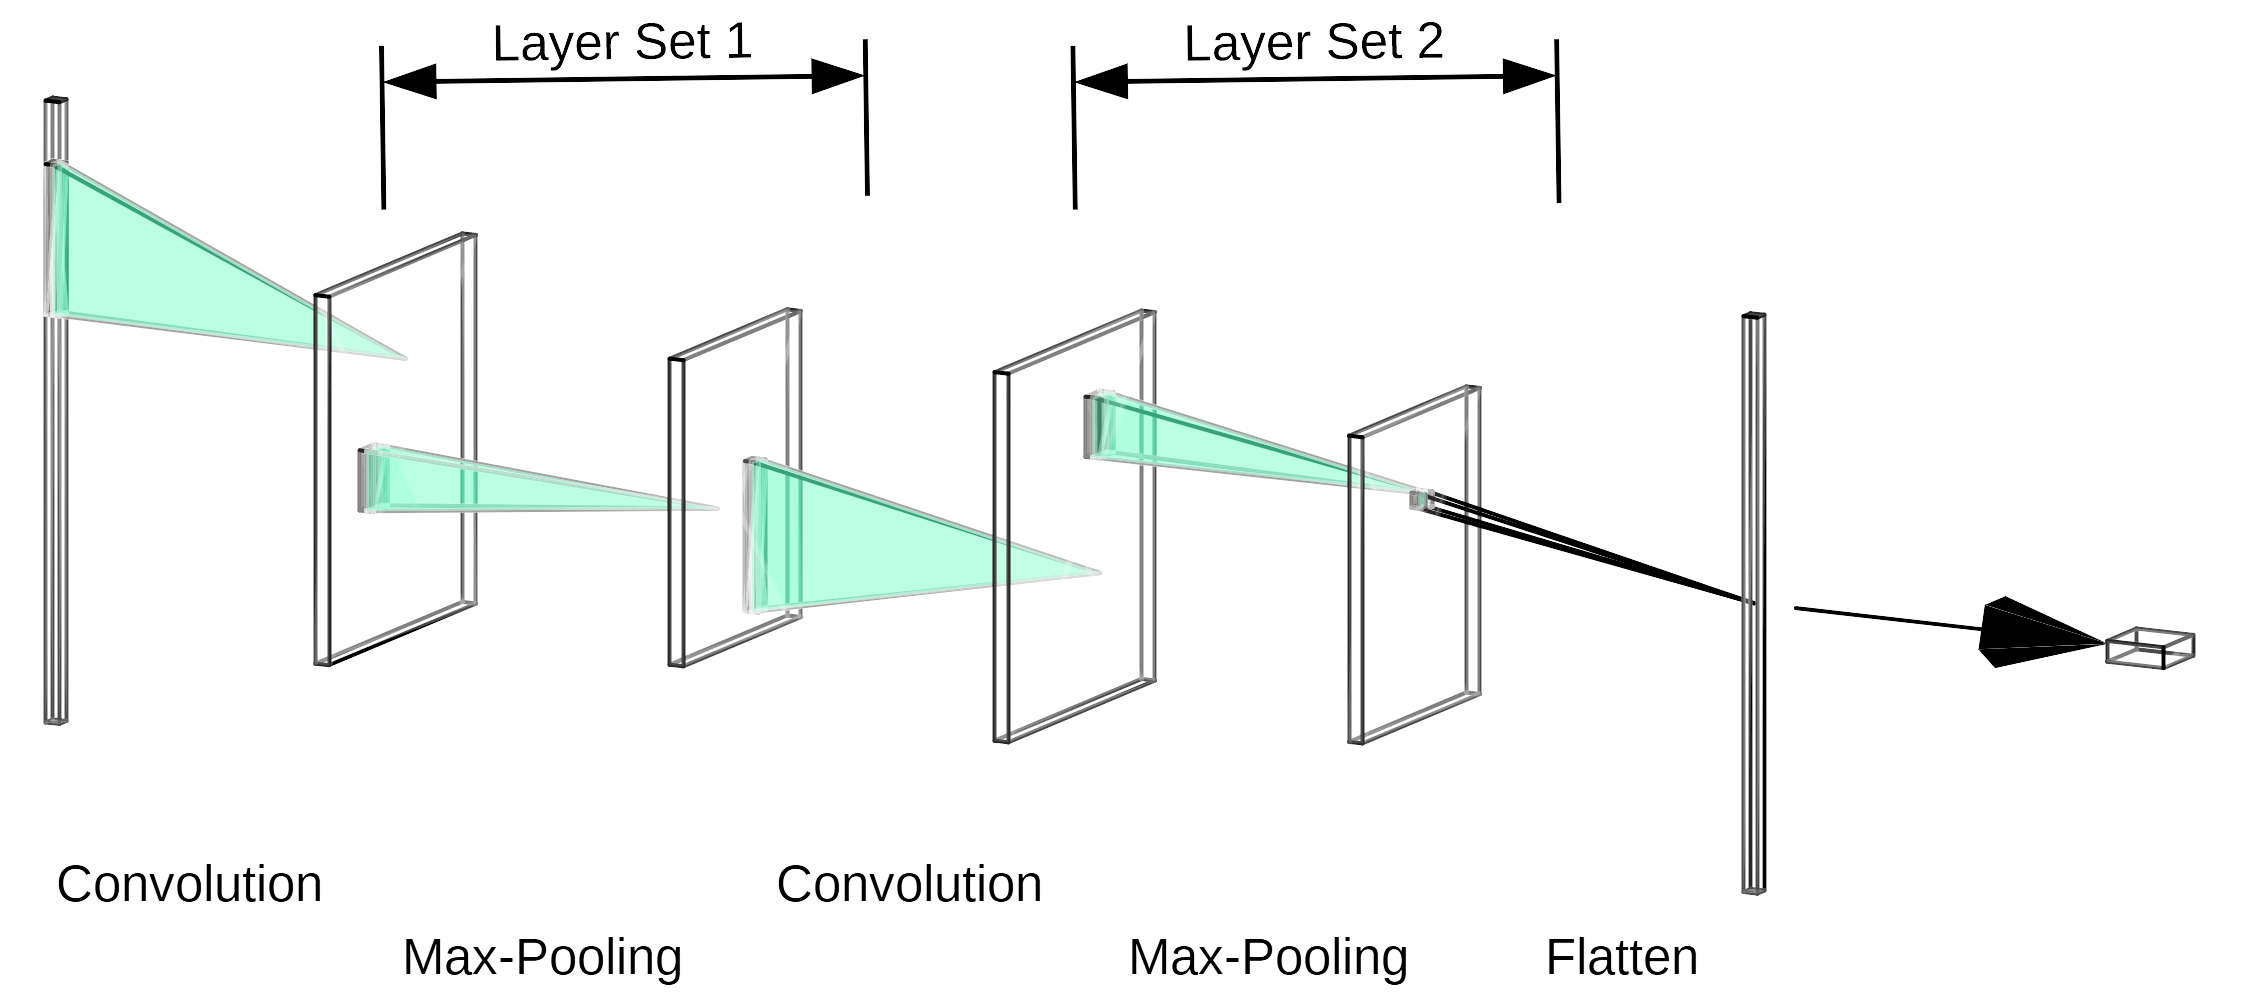
\includegraphics[width=0.8\linewidth]{image/nn.png}
\caption{1D-CNN with 2 convolution layer set.}
\label{1dCNN}
\end{figure}

Other CNNs implemented with \emph{Pytorch}\cite{NEURIPS2019_9015} can also be analyzed with \emph{Odysseia} but training protocol need to be clarifed by user in advance.
\end{itemize}

Eighty-one model builds consisting of 1 SVC, 16 GBTrees, and 64 CNNs will be used to initialize vanilla models with default model config file.
In each training iteration, each vanilla classifier will be fed with same set of pseudo-cGRNs as training samples and is primarily assessed according to prediction accuracy on untrained pseudo-cGRNs.
By default setting, 70\% of pseudo-cGRNs will be split into training set while 30\% will be split into testing set at each iteration.
The classifiers capable of passing accuracy threshold will be kept for further comparisons with other classifers trained with different sample sets in later iterations.

At the end of this step, all available pseudo-cGRNs will be joint to use as testing data, and all candidate classifers will be evaluated on their prediction accuracies of fully joint testing data.
Considering that the real random choice can reach an accuracy of 50\% in binary classification question, the accuracy threshold for either local accuracy test or fully joint data test is set to 90\%.

\begin{figure}[ht]
\centering
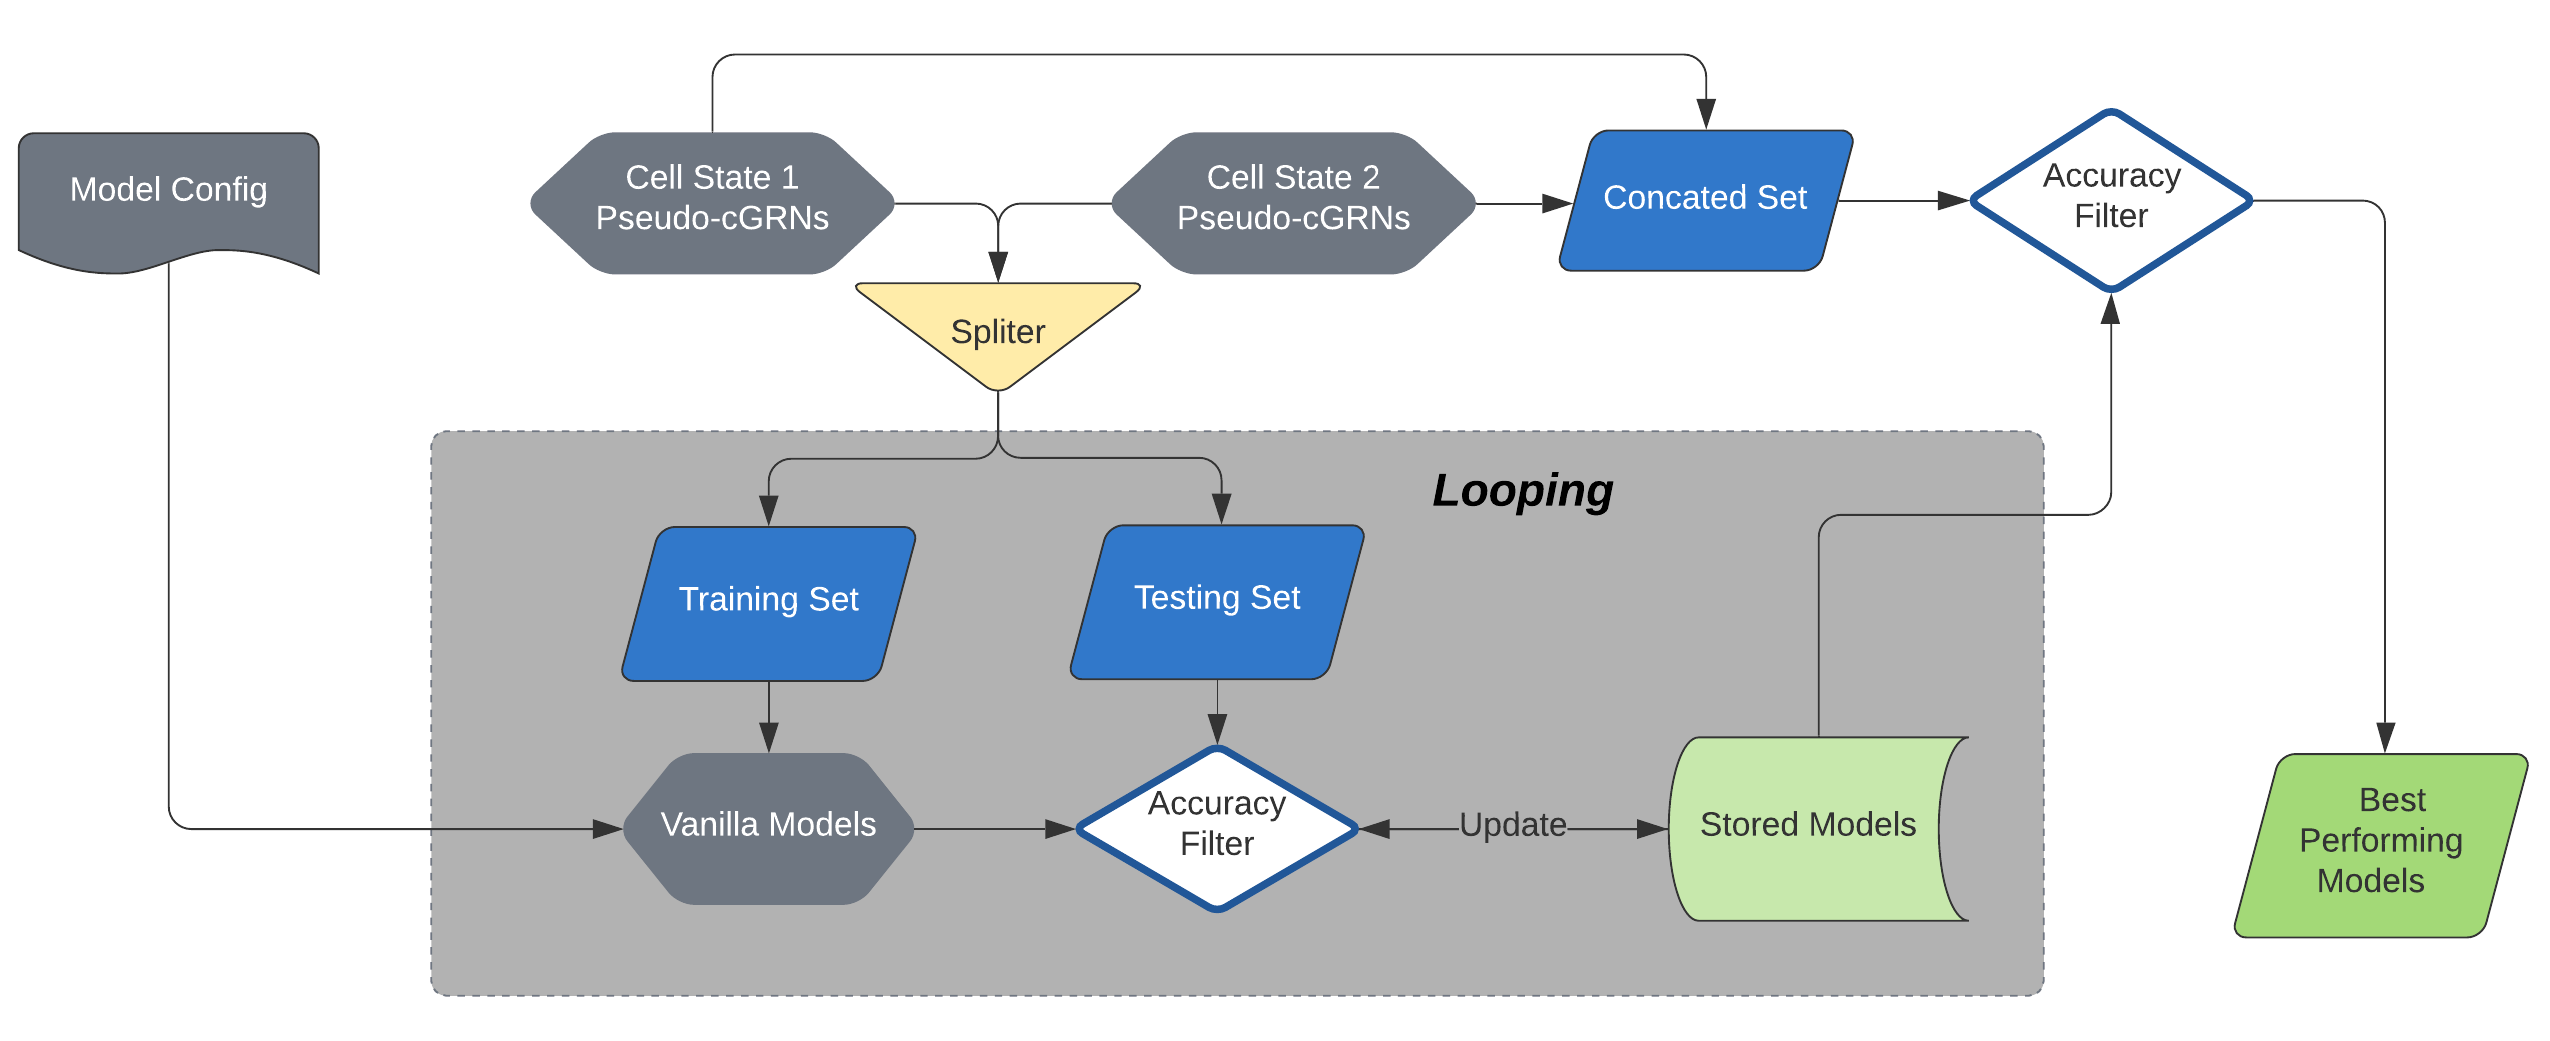
\includegraphics[width=1.0\linewidth]{image/Odysseus.png}
\caption{
Workflow to generate well-performing classifers.
\textbf{\emph{(1)}} In each training iteration, input pseudo-cGRNs will be split into training set and testing set according to given ratio.
By default, the ratio is set to 70\% for training and 30\% for testing.
\textbf{\emph{(2)}} According to given classification model config file, vanilla classifiers will be initialized and trained with training set.
The predictive accuracy of classifiers will be pre-assessed with testing data.
Classifers reaching accuracy threshold, which is set to 0.9 by default, will be kept for further accuracy assessment in further training iterations.
\textbf{\emph{(3)}} After all training iterations, all pseudo-cGRNs will be concatenated as one testing set to assess accuracies of classifers being kept.
Classifers reach accuracy threshold, set to 0.9 by default, will be passed to further analysis.
}
\label{odysseus}
\end{figure}

\subsection*{Step 3: Classifier interpretation}
\label{step3}
During the last accuracy assessment in Step 2, all classifer's predictions consisting with ground truths will be marked with corresponding input pseudo-cGRNs.
Briefly, in this step, \emph{Odysseia} interprets how well-performing classifiers make correct predictions on CS categories of given pseudo-cGRNs.
Integrating interpretations of all well-performing classifers, the generalized importance values of features, which are represented by GRPs in \emph{Odysseia}'s scenario, in determining CS can be approached.

Several packages already have internalized methods implemented for machine learning models to analyze feature importance.
For example, GBTree implemented with \emph{XGBoost}\cite{chen2016xgboost} can have feature importance approached through calculating by average weight gain at each split involving the feature, and linear SVC implemented with \emph{scikit-learn}\cite{scikit-learn} can have the importance approached with feature coefficient.
Regarding the standard differences between these internalized methods, we utilize \emph{softmax} function to normalize feature importance and define the normalized importance calculation function as:

\centerline{$\textit{T(Z) = }\left\{\frac{f(Z_i)}{\sum_{j = 1}^{L} f(Z_j)}\right\}, i \in Z$}

\noindent Here $Z$ is feature set; $L$ is total number of features; $f(X)$ is internalized  feature importance calculating function of classification model.\

However, for numerous machine learning models, there is no internalized feature importance approaching method, for example, NN-based models implemented with Pytorch\cite{NEURIPS2019_9015} or generalized method cannot be appropriately applied with selected models such as Kernelized SVC implement with \emph{scikit-learn}\cite{scikit-learn}.
Therefore, we apply the concept of The Shapley value\cite{roth_1988} to build an universal approach for determining importance of each feature in any kind of machine learning model.
Specific Shapley value calculation or approaching methods are implemented with \emph{SHAP}\cite{lundberg2017unified} and applied to different types of classifiers as shown in Table\ref{shap}.

\begin{table}[ht]
\centering
\begin{tabular}{|l|l|l|}
\hline
\textbf{Model Genera} & \textbf{Model Example} & \textbf{SHAP\cite{lundberg2017unified} Method}  \\
\hline
Tree-Based & GBTree & Tree Explainer \\
\hline
NN-Based without Repetitive Layer Sets & CNN & Deep Explainer \\
\hline
NN-Based with Repetitive Layer Sets & Recurrent Neural Network & Gradient Explainer \\
\hline
Kernel Machines & SVC & Kernel Explainer \\
\hline
Linear Models & Logistic Regression & Linear Explainer \\
\hline
\end{tabular}
\caption{\label{shap}Machine learning model generas with applicable Shapley value approaching methods}
\end{table}

Let $N$ denotes the total number of correct predictions, $\phi_{x,j}^{i}$ and $\phi_{y,j}^{i}$ denotes Shapley value of feature $i$ when predicting sample $j$ as type $x$ or type $y$, the function determining importance values of feature set $z$ can be expressed as:

\centerline{$\textit{T(Z) = softmax}(\left\{\sum_{j = 1}^{N}\frac{\left|\phi_{x,j}^{i}\right| + \left|\phi_{y,j}^{i}\right|}{2}\right\}, i \in Z)$}

Following the analysis of all classifers, each feature's general importance value can be obtained through:

\centerline{$g(i) = \sum_{j = 1}^{C}T_{j}(Z)[i]$}

Here $i$ denotes i\emph{th} feature or GRP, $C$ denotes the total number of classifers being analyzed, $T_{j}(Z)[i]$ denotes i\emph{th} feature's importance value calculated through analyzing j\emph{th} classifier.

\subsection*{Step 4: Key genes extraction}
\label{step4}
With feature list ranked according to importance values, \emph{Odysseia} reconstructs a regulon for top-ranked GRPs and extracts influential genes among the regulon.
If analoging regulon or GRN with the graph concept in discrete mathematics, one of the most common methods to analyze influence of a vertex, which is equivalent to a gene, is assessing correspond degree of the vertex.
Although the regulatory source and target within a GRP can be determined by utilizing interaction database such as \emph{GTRD}\cite{gkaa1057}, shows regulatory relationship of interactors, numerous computational prediction methods, for example,  \emph{GRNBoost2}\cite{grnboost2}, and comprehensive interaction database, for example, \emph{BioGRID}\cite{biogrid}, could not provide faithful indication on regulatory directions.
Consequently, based on choice of interaction database for \emph{Odysseia}, the regulon reconstructed cannot be guaranteed to be a directed graph, but can surely be analyzed as an undirected graph.
Therefore, in this step, \emph{odysseia} primarily extracts genes with high degrees in the regulon, regardless of they are in-degree or out-degree.
To limit total amount of output key genes, the default setting of \emph{Odysseia} reconstructs regulon for top 100 GRPs, and genes with degree higher than two in the regulon will be considered influential.
If regulatory relationships can be clarifed, the regulatory sources capable of regulating multiple key genes and the regulatory targets influenced by multiple key genes can also be extracted according to GRN reconstruction guidance.

In the circumstance of finding genes potentially inducing CS conversion, referred as \emph{Mogrify}\cite{mogrify_2016}, genes either CS deterministic or capable of regulating key genes shall gain attention.
If a gene is not marked as "important", it must be capable of regulating more than 2 listed key genes to be considered as an important regulatory interactor.

% Both non-convergence issue and feature lost issue reflect on one of the key problems for $AutoML$: "No single machine learning method performs best on all datasets".\cite{NIPS2015_11d0e628}
% Even though this problem can be solved while viewing $AutoML$ as a $CASH$ problem \cite{thornton2013auto}, such approach may not be directly deployable in our scenario considering comprehensive CS deterministic GFs or GRPs could be hardly labeled out.
% Hence, in contrast with directly automating key features finding process, we decide to partially automate CS classification process and export candidate components of joint algorithm to feature importance analysis.
% Compared with applying a particular $ML$ model, $CASH$ solving process during automation have higher potential to utilize comprehensive key features instead limited set of them.
% Furthermore, due to the network-based essence of \emph{Odysseia}, some CS deterministic features failed to be detected after classification model analysis, if having close regulatory relationships with multiple confirmed GFs, can still be traced down during regulon-based analysis at post stage analysis.
%
% \subsection*{Construct Pipeline with Odysseia Modules}
% Utilizing modules stated above, a generalized feature extraction pipeline, $Homeros$ which can be summarized as Figure \ref{odysseia}, has been built.
% At first stage of $Homeros$, a $GRN$ reconstruction guidance will be cast with all available data applying $Kirke$ module.
% Next, $Odysseus$ will be initialized with model config file and train out well-performing models for $CL$ classification.
% Models output by $Odysseus$ will then be analyzed with $Penelopeia$ module to propose important GFs and associated GRPs.
% According to changes in abundant GFs among significant GRPs found by $Penelopeia$, program will determine whether another iteration of training or early stopping shall be performed.
% Once looping part either reaches iteration time limit or be early stopped, latest feature importance table will be used to finalize abundant GFs.
% Finally, regulon analysis will find common source regulators and targeting genes of the abundant GFs and generate candidate GF table.

\section*{Results}
\label{res}
In order to evaluate analytic power, we tested \emph{Odysseia} with three previously published CS conversion related scRNA-seq datasets.
Considering the differences in information availability and data size among datasets, each dataset is analyzed with adjusted process:
\begin{itemize}
\setlength\itemsep{0em}
\item \textbf{MEF and ESC}:
This dataset was used to study cell fate continuum when reprogramming MEF into iPSC, one of the most well-studied CS conversions.\cite{mef_ipsc_cas}
To simulate the process of finding gene combination for reprogramming somatic cell into pluripotent stem cell, we used scGEPs-labeled MEFs and embryonic stem cells(ESCs) as input of \emph{Odysseia}.
Due to the limited amount of scGEPs, SWA with window size set to 10 and padding stride set to 1 was applied to generate 73 ESC pseudo-cGEPs and 65 MEF pseudo-cGEPs.
Std threshold is set to 100, which resulted in GRN reconstruct guidance consisting 72440 GRPs, considering the computational load our testing device could accept.
While all other parameters remained as default, \emph{Odysseia} extracted 16 key genes and 9 common regulatory sources of key genes.
Partial key genes which have already been reported in other studies are listed below, and complete output gene list is included in \textbf{Supplementary Table 1}.

\begin{table}[ht]
\centering
\begin{tabular}{|l|l|l|l|}
\hline
\textbf{Gene} & \textbf{Occurrence} & \textbf{Degree} & \textbf{Previous report}  \\
\hline
Nanog & 16 & 0 & Can reprogram MEF into iPSC with other GFs\cite{ips7f, oct4_nanog_sox2_lin28, oct4_nanog_sox2} \\
\hline
Esrrb & 10 & 0 & Can reprogram MEF into iPSC with other GFs\cite{ips7f, LIF_esrrb, gtmEsrrb_iPSC, JARID2_PRDM14_ESRRB_SALL4A} \\
\hline
Sall4 & 10 & 0 & Can reprogram MEF into iPSC with other GFs\cite{ips7f, JARID2_PRDM14_ESRRB_SALL4A} \\
\hline
Tfcp2l1 & 8 & 0 & Key regulatory mediator supporting ESC identity\cite{tfcp2l1_1, tfcp2l1_2} \\
\hline
Pou5f1 (Oct4) & 7 & 0 & Can reprogram MEF into iPSC with other GFs\cite{yamanaka_2006, oct4_nanog_sox2_lin28, oct4_nanog_sox2, ips2f, ipsOK, osk} \\
\hline
Fos & 3 & 2 & Subunit of AP-1 which can prohibit iPSC reprogramming\cite{ips7f, ipsAP1} \\
\hline
Klf4 & 2 & 0 & Can reprogram MEF into iPSC with other GFs\cite{yamanaka_2006, ips2f, ipsOK, osk} \\
\hline
\end{tabular}
\end{table}

Here, \textbf{Occurrence} refers to occurrences in top ranked GRPs; \textbf{Degree} refers to amount of regulating key genes; \textbf{Previous report} summarizes key findings from previous reports.

\item \textbf{MEF and iMPC}:
The main purpose of analyzing this dataset is to assess \emph{Odysseia}'s performance while stimulating natural cells with artificially induced cells.
This dataset is retrieved from research project studying detailed processes of fibroblast to myocyte and myogenic progenitor cell(MPC) conversion.\cite{mef_iMPC_ETH}
For approaching muscle cell reprogramming, the output goal of this analysis is designed to find key genes for converting MEF into myoblast and further derived myotube can be stimulated with MyoD+ induced MPCs(iMPCs)\cite{mpc_as_myoblast}.
Practically, only iMPC scGEPs with EL of Myod1 greater than 1, the lowest positive EL in dataset, were extracted as myoblasts and myotubes co-culture and analyzed with MEF scGEPs.
Due to computational limitation on our device, pseudo-cGEPs were generated with every 100 scGEPs.
As a result, in total of 99 MyoD+ iMPC and 62 MEFs pseudo-cGEPs were generated.
Std threshold was also set to 5 to limit the size of GRN reconstruct guidance to be 3756 GRPs.
Without any change on other default parameters, \emph{Odysseia} extracted 6 key genes and 3 common regulatory sources of key genes.
Partial analysis result is listed below under same format as mentioned in section above, and complete output gene list is included in \textbf{Supplementary Table 2}.

\begin{table}[ht]
\centering
\begin{tabular}{|l|l|l|l|}
\hline
\textbf{Gene} & \textbf{Occurrence} & \textbf{Degree} & \textbf{Previous report}  \\
\hline
Sox4 & 73 & 2 & Myogenesis mediator\cite{sox4_2013, myogenic_repro_2018} \\
\hline
Mef2c & 23 & 3 & Synergy factor of MyoD in the conversion of MEF into myoblast\cite{mef2_2017, mef2_skeletal}\\
\hline
Myog & 2 & 4 & Marker of differentiating myoblast\cite{myog_1996, myog_2017} \\
\hline
Tcf4 & 2 & 2 & Marker of MEF in muscle connective tissue; Myogenesis mediator\cite{tcf4_2011, tcf4_2016, tcf4_2017}\\
\hline
Mef2a & 0 & 3 & Synergy factor of MyoD in the conversion of MEF into myoblast\cite{mef2_2017, mef2_skeletal}\\
\hline
Myod1 & 0 & 3 & Can reprogram MEF into myoblast and myotube solely\cite{mef_iMPC_ETH, myod_1990, myod_crispr} \\
\hline
\end{tabular}
\end{table}

\item \textbf{Radial glia and Neuron}:
Furthermore, contemplating feasible difficulty in obtaining purified scRNA-seq dataset of cell subtypes, we tested \emph{Odysseia} when analyzing differences between purified and mixed CS data.
The input dataset of this analysis consists of scGEPs of purified neuron and iPSC-derived radial glial cell, the progenitor cell of neuron, mixing with neuron.
All of the data are retrieved from published dataset used to examine CS conversion from iPSC to neuron.\cite{ips_neuron_ascl1}
Similar with MEF and iMPC analysis, pseudo-cGEPs were also generated with every 100 scGEPs which result in a total of 90 neural co-culture and 72 purified neuron pseudo-cGEPs.
Without changes on other default parameters, 40441 GRPs were included in GRN reconstruct guidance, and \emph{Odysseia} extracted 17 key genes and 19 common regulatory sources of key genes.
Partial analysis result is listed below under same format as mentioned in section above, and complete output gene list is included in \textbf{Supplementary Table 3}.

\begin{table}[ht]
\centering
\begin{tabular}{|l|l|l|l|}
\hline
\textbf{Gene} & \textbf{Occurrence} & \textbf{Degree} & \textbf{Previous report}  \\
\hline
Ets2 & 48 & 12 & Cell cycle regulator need to be repressed for primary neurogenesis\cite{ets2_1, ets2_2} \\
\hline
Isl1 & 23 & 4 & Key gene for motor neuron development\cite{isl1_1, isl1_2011, isl1_repro}\\
\hline
Ascl1 & 16 & 13 & Key neurogenesis regulator\cite{ips_neuron_ascl1, ascl1_1}; Can induce neuronal reprogramming solely\cite{ascl1_1frepro ,ascl1_repro} \\
\hline
Nr3c1 & 0 & 9 & Cell cycle inhibitor during embryonic neurogenesis\cite{nr3c1}\\
\hline
Rbpj & 0 & 8 & Key mediator of Notch signaling in neurogenesis\cite{rbpj_1, rbpj_2, rbpj_3}\\
\hline
Neurod1 & 0 & 7 & Key neurogenesis regulator\cite{ips_neuron_ascl1, neurod1_1, neurod1_2, neurod1_3, neurod1_4} \\
\hline
\end{tabular}
\end{table}

\end{itemize}

Even though \emph{Odysseia} is unable to guarantee a gene combination inducing CS conversion, numerous previously discovered key genes can be successfully extracted, which indicated gene combination known capable to convert CSs.
For example, when analyzing MEF with iPSC, the top three genes having most occurrences among important GRPs are determined as key factors to reprogram MEF into iPSC with 7F combination\cite{ips7f}.
With Jdp2, which is selected to block AP-1 activity also as Fos indicated, the combination of Jdp2, Nanog, Esrrb, and Sall4 is demonstrated as a minimum 4F functional set to perform cell reprogramming\cite{ips7f}.
While Sall4 indicated interaction between Sox2 and Oct4\cite{sall4_oct4_sox2}, main components among Yamanaka factors\cite{yamanaka_2006, osk} can also be extracted with \emph{Odysseia}'s analysis result.
Between MEF and muscle cell, multiple works demonstrated capability of Myod1, which is successfully extracted by \emph{Odysseia}, in artificially induce CS conversion.\cite{myod_1990, myod_crispr}
For neurogenesis analysis, Ascl1, included as key factor in several neuronal conversion methods\cite{ascl1_repro,  ascl1_1frepro}, is marked as key gene with the most consequential regulatory influence by \emph{Odysseia}.
It is noteworthy that other factors extracted with \emph{Odysseia} may also play an important role in CS conversions but have not yet been  testified with adequate experiments.


\section*{Discussion}
\label{disc}
As scRNA-seq technology becomes increasingly accessible and applicable, an efficient and robust analytical system capable of extracting key GFs differentiating CSs will also become highly demanded.
In this paper, we showed \emph{Odysseia}'s applicability in analyzing scRNA-seq derived data for further CS-related research.
According to test cases so far, key genes significant enough to induce CS conversions appear to have either high occurrence in top ranked GRPs or high regulatory influence on other key genes.
Without any previous knowledge on studying CSs, Gene Ontology (GO) enrichment analysis can potentially narrow down key cellular functions changed in different CSs.

However, further tests and optimizations are necessary to confirm \emph{Odysseia}'s applicability on guiding frontier researches.
While more resources become available, other classification models and interpretation methods will be added and tested with current version on larger scales.
Further optimized model selection process will also be critical to improve system's overall performance.

With result achieved so far, we anticipate that \emph{Odysseia} will become useful in providing insightful advices on not only learning differences between CSs and cell subtypes, but also finding key GFs to induce CS conversions unachievable so far.

% \section*{Conclusion}
% \label{conc}
% Conclusion goes here

\bibliography{reference}

% For data citations of datasets uploaded to e.g. \emph{figshare}, please use the \verb|howpublished| option in the bib entry to specify the platform and the link, as in the \verb|Hao:gidmaps:2014| example in the sample bibliography file.

\section*{Author contributions statement}
\textbf{J.Y.}: Methodology, Software, Writing- Original draft preparation
\textbf{J.T.}: Writing - Review \& Editing
% J.W.: Project administration

\section*{Additional information}
All scRNA-seq datasets are retrieved from Gene Expression Omnibus(GEO) as described in Key Resource Table below.


\subsection*{Key Resource Table}

\begin{tabular}{|l|l|l|}
\hline
\textbf{Resource}                      & \textbf{Source}                              & \textbf{Usage}                                                                                                                  \\ \hline
MEF and ESC scRNA-seq data             & GEO Accession: GSE103221 & \begin{tabular}[c]{@{}l@{}}Samples with label started with 'mef' as MEF\\ Samples with label started with 'esc' as ESC\end{tabular} \\ \hline
MEF and iMPC scRNA-seq data            & GEO Accession: GSE169054 & \begin{tabular}[c]{@{}l@{}}GSM5175907 as iMPC\\ GSM5643793 as MEF\end{tabular}                                                  \\ \hline
Radial glia and Neuron scRNA-seq data & GEO Accession: GSE185275 & \begin{tabular}[c]{@{}l@{}}GSM5609927 as neural co-culture\\ GSM5609930 as purified neurons\end{tabular}                        \\ \hline
\end{tabular}


% $CASH$        & Combined Algorithm Selection and Hyperparameter optimization\\
\end{document}
